\chapter{Portfolio Allocation}
\section{Introduction}

In the past chapter, we looked at simple models of the risk-return trade-off, however models can be more complex for a single security. This chapter goes through the CAPM or Capital Asset Pricing Model, which is a model that describes the relationship between risk and expected return.

\begin{definitionbox}{Definition of Portfolio Allocation}
    Portfolio allocation refers to the distribution of an individual's investment across different asset classes, such as stocks, bonds, and real estate, with the aim of maximising returns while minimising risk.
\end{definitionbox}

\section{Portfolio Theory}
When calculating the return and volatility of a two-stock portfolio, we consider the weighted average of the returns and variances based on the allocation of the two stocks, where $x_i$ is the weight of the portfolio invested in asset $i$ and $R_i$ is the return of asset $i$. Note that the weights $x_A, x_b$ must sum to 1.

\begin{equation}
    R_p = x_AR_A + x_BR_B
\end{equation}

Denote the volatilities of the two assets as $\sigma_A, \sigma_B$ and the correlation between the two assets as $\rho_{AB}$. The volatility of the portfolio is given by:

\begin{equation}
    \sigma_p = \sqrt{\underbrace{x_A^2\sigma_A^2}_{\text{A's individual contribution to vol}} + \underbrace{x_B^2\sigma_B^2}_{\text{B's individual contribution to vol}} + \underbrace{2x_Ax_B\sigma_A\sigma_B\rho_{AB}}_{\text{Covariance between A and B}}}
\end{equation}

Changing portfolio weights can change the risk-return profile of the portfolio. 

Assume we have a portfolio of Coca-Cola and Intel.

\begin{table}[ht]
    \centering
    \caption{Expected Returns and Volatility for Intel and Coca-Cola}
    \label{tab:intel-coke}
    \begin{tabular}{@{}lcc@{}}
    \toprule
    \textbf{Company} & \textbf{E(R)} & \textbf{Vol} \\
    \midrule
    Intel    & 26\% & 50\% \\
    Coca-Cola & 6\%  & 25\% \\
    \midrule
    \multicolumn{3}{c}{Correlation = 0} \\
    \bottomrule
    \end{tabular}
 \end{table}

Table \ref{tab:intel-coke} shows possible weight allocations for Coca-Cola and intel. Note that the variance of the portfolio is not a weighted average of the variances of the two stocks, because of the added covariance term. Since these patterns may not be intuitive, it is best to visualise portfolios with a graph to show the \textbf{efficient frontier}


\begin{table}[ht]
    \centering
    \caption{Portfolio Expected Return and Standard Deviation}
    \begin{tabular}{@{}cccc@{}}
    \toprule
    \textbf{Xi} & \textbf{Xc} & \textbf{E(Rp)} & \textbf{SD(Rp)} \\ 
    \midrule
    1    & 0    & 26.00\% & 50.00\% \\
    0.98 & 0.02 & 25.60\% & 49.00\% \\
    0.88 & 0.12 & 23.60\% & 44.10\% \\
    0.78 & 0.22 & 21.60\% & 39.39\% \\
    0.68 & 0.32 & 19.60\% & 34.93\% \\
    0.58 & 0.42 & 17.60\% & 30.84\% \\
    0.48 & 0.52 & 15.60\% & 27.29\% \\
    0.38 & 0.62 & 13.60\% & 24.52\% \\
    0.28 & 0.72 & 11.60\% & 22.80\% \\
    0.18 & 0.82 & 9.60\%  & 22.39\% \\
    0.08 & 0.92 & 7.60\%  & 23.35\% \\
    0    & 1    & 6.00\%  & 25.00\% \\
    \bottomrule
    \end{tabular}
    \end{table}



Diversification can reduce some risk without compromising on returns (making an efficient portfolio). 

\begin{figure}[H]
    \centering
    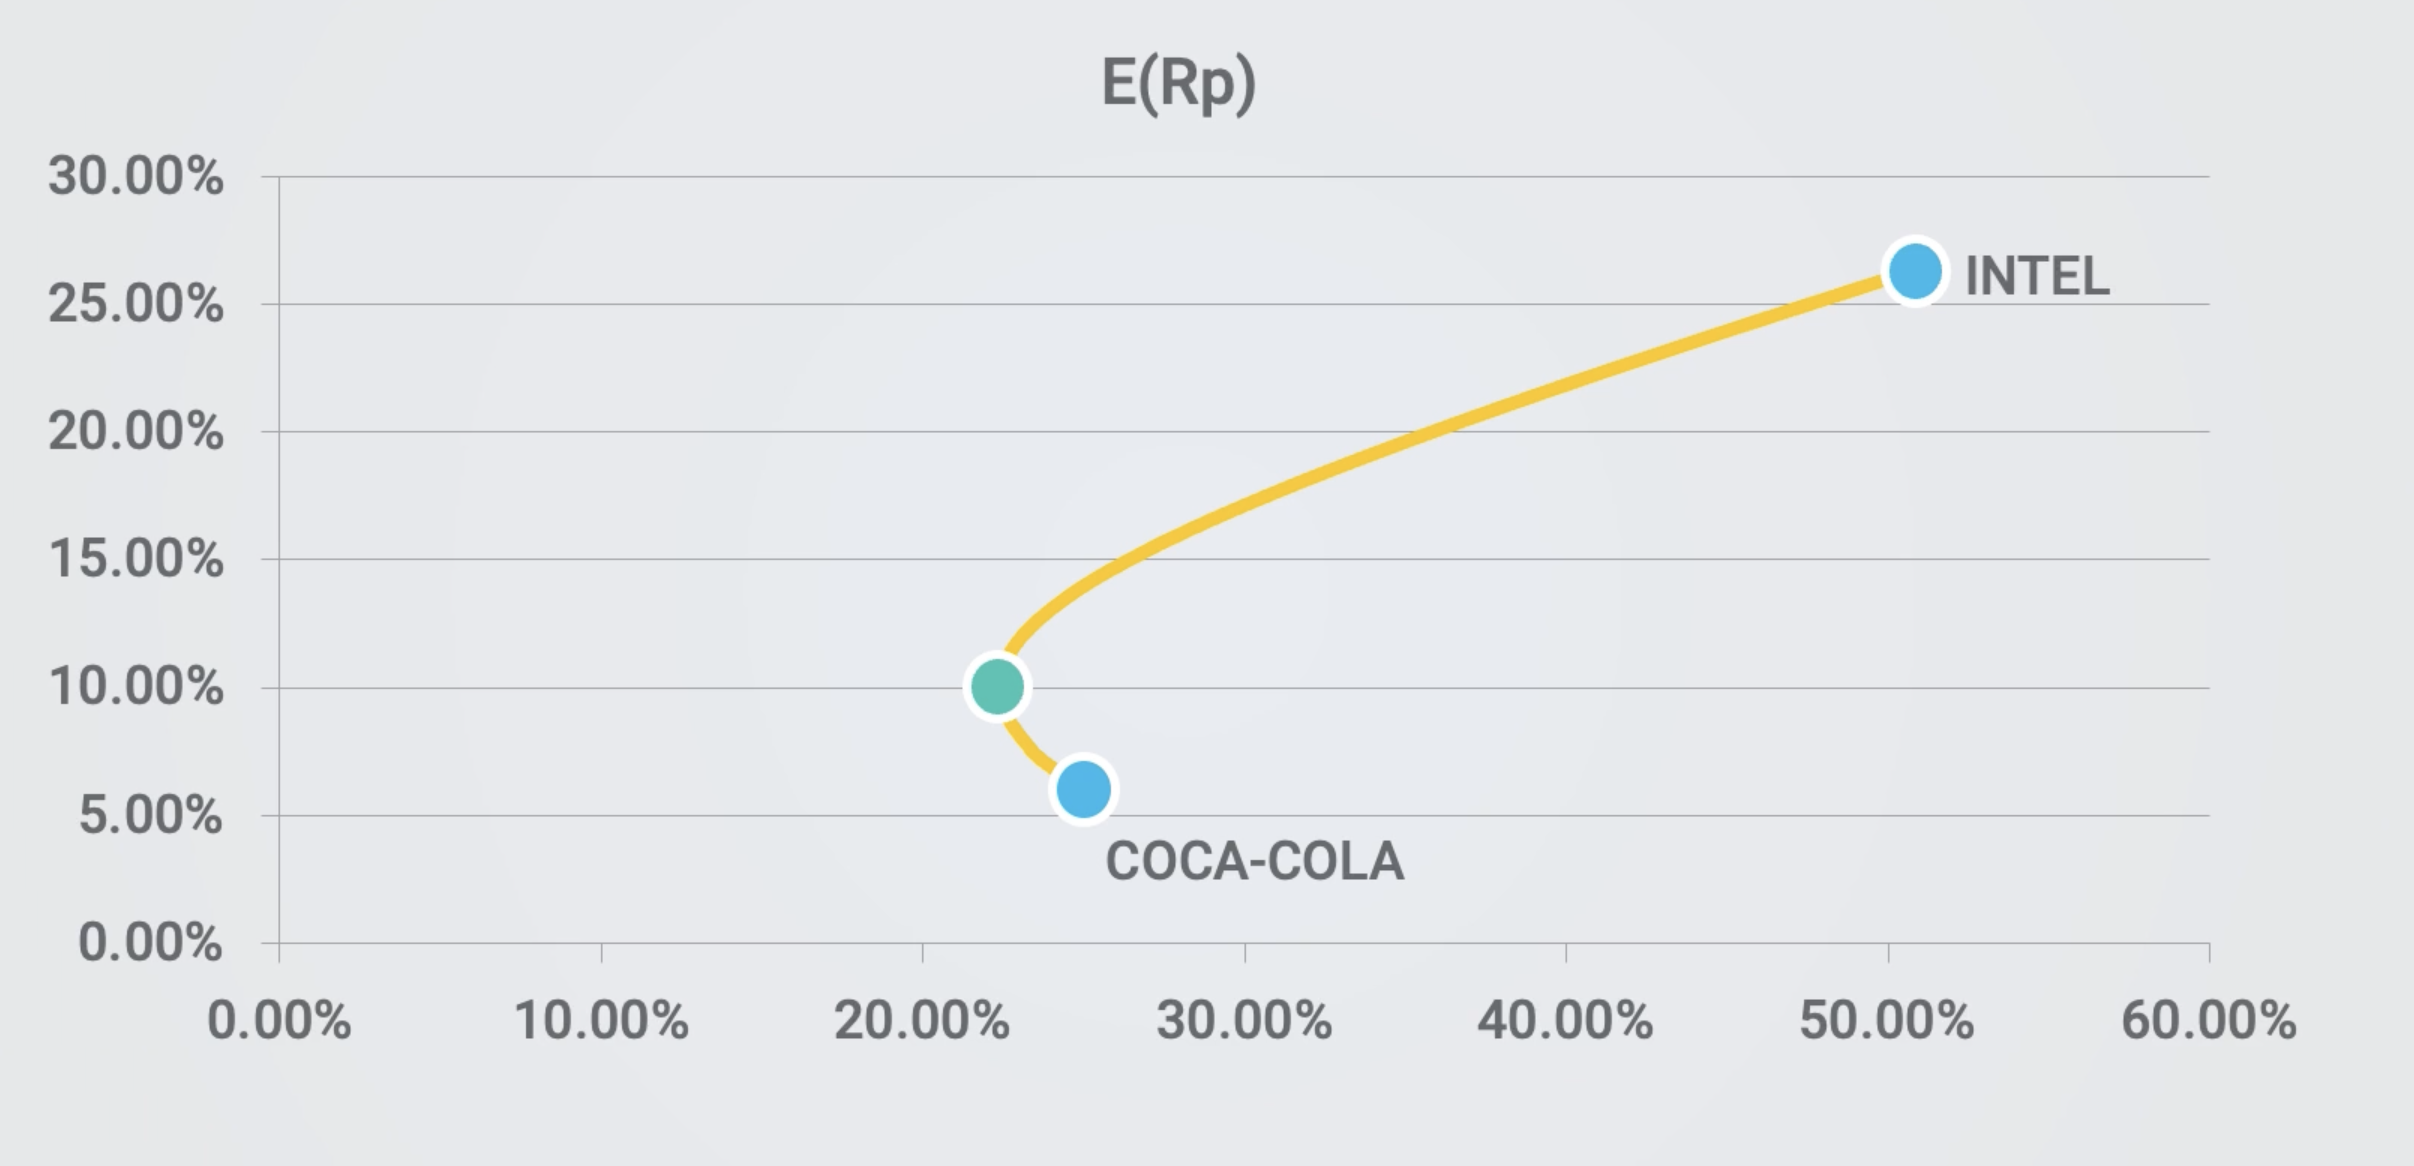
\includegraphics[width=0.8\textwidth]{img/6.2.1.png}
    \caption{Efficient Frontier}
    \label{fig:efficient_frontier}    
\end{figure}

Notice that COCA-COLA by itself has a lower return and lower risk than if it was slightly supplemented by Intel, where risk is reduced to a minimum but returns are slightly higher, thus an efficient portfolio. An efficient portfolio is one that has the highest return for a given level of risk, or the lowest risk for a given level of return.\\

Return correlation is a measure of how two assets move together. A correlation of 1 means that the two assets move in the same direction, while a correlation of -1 means that the two assets move in opposite directions. A correlation of 0 means that the two assets are independent of each other.\\

\begin{figure}[H]
    \centering
    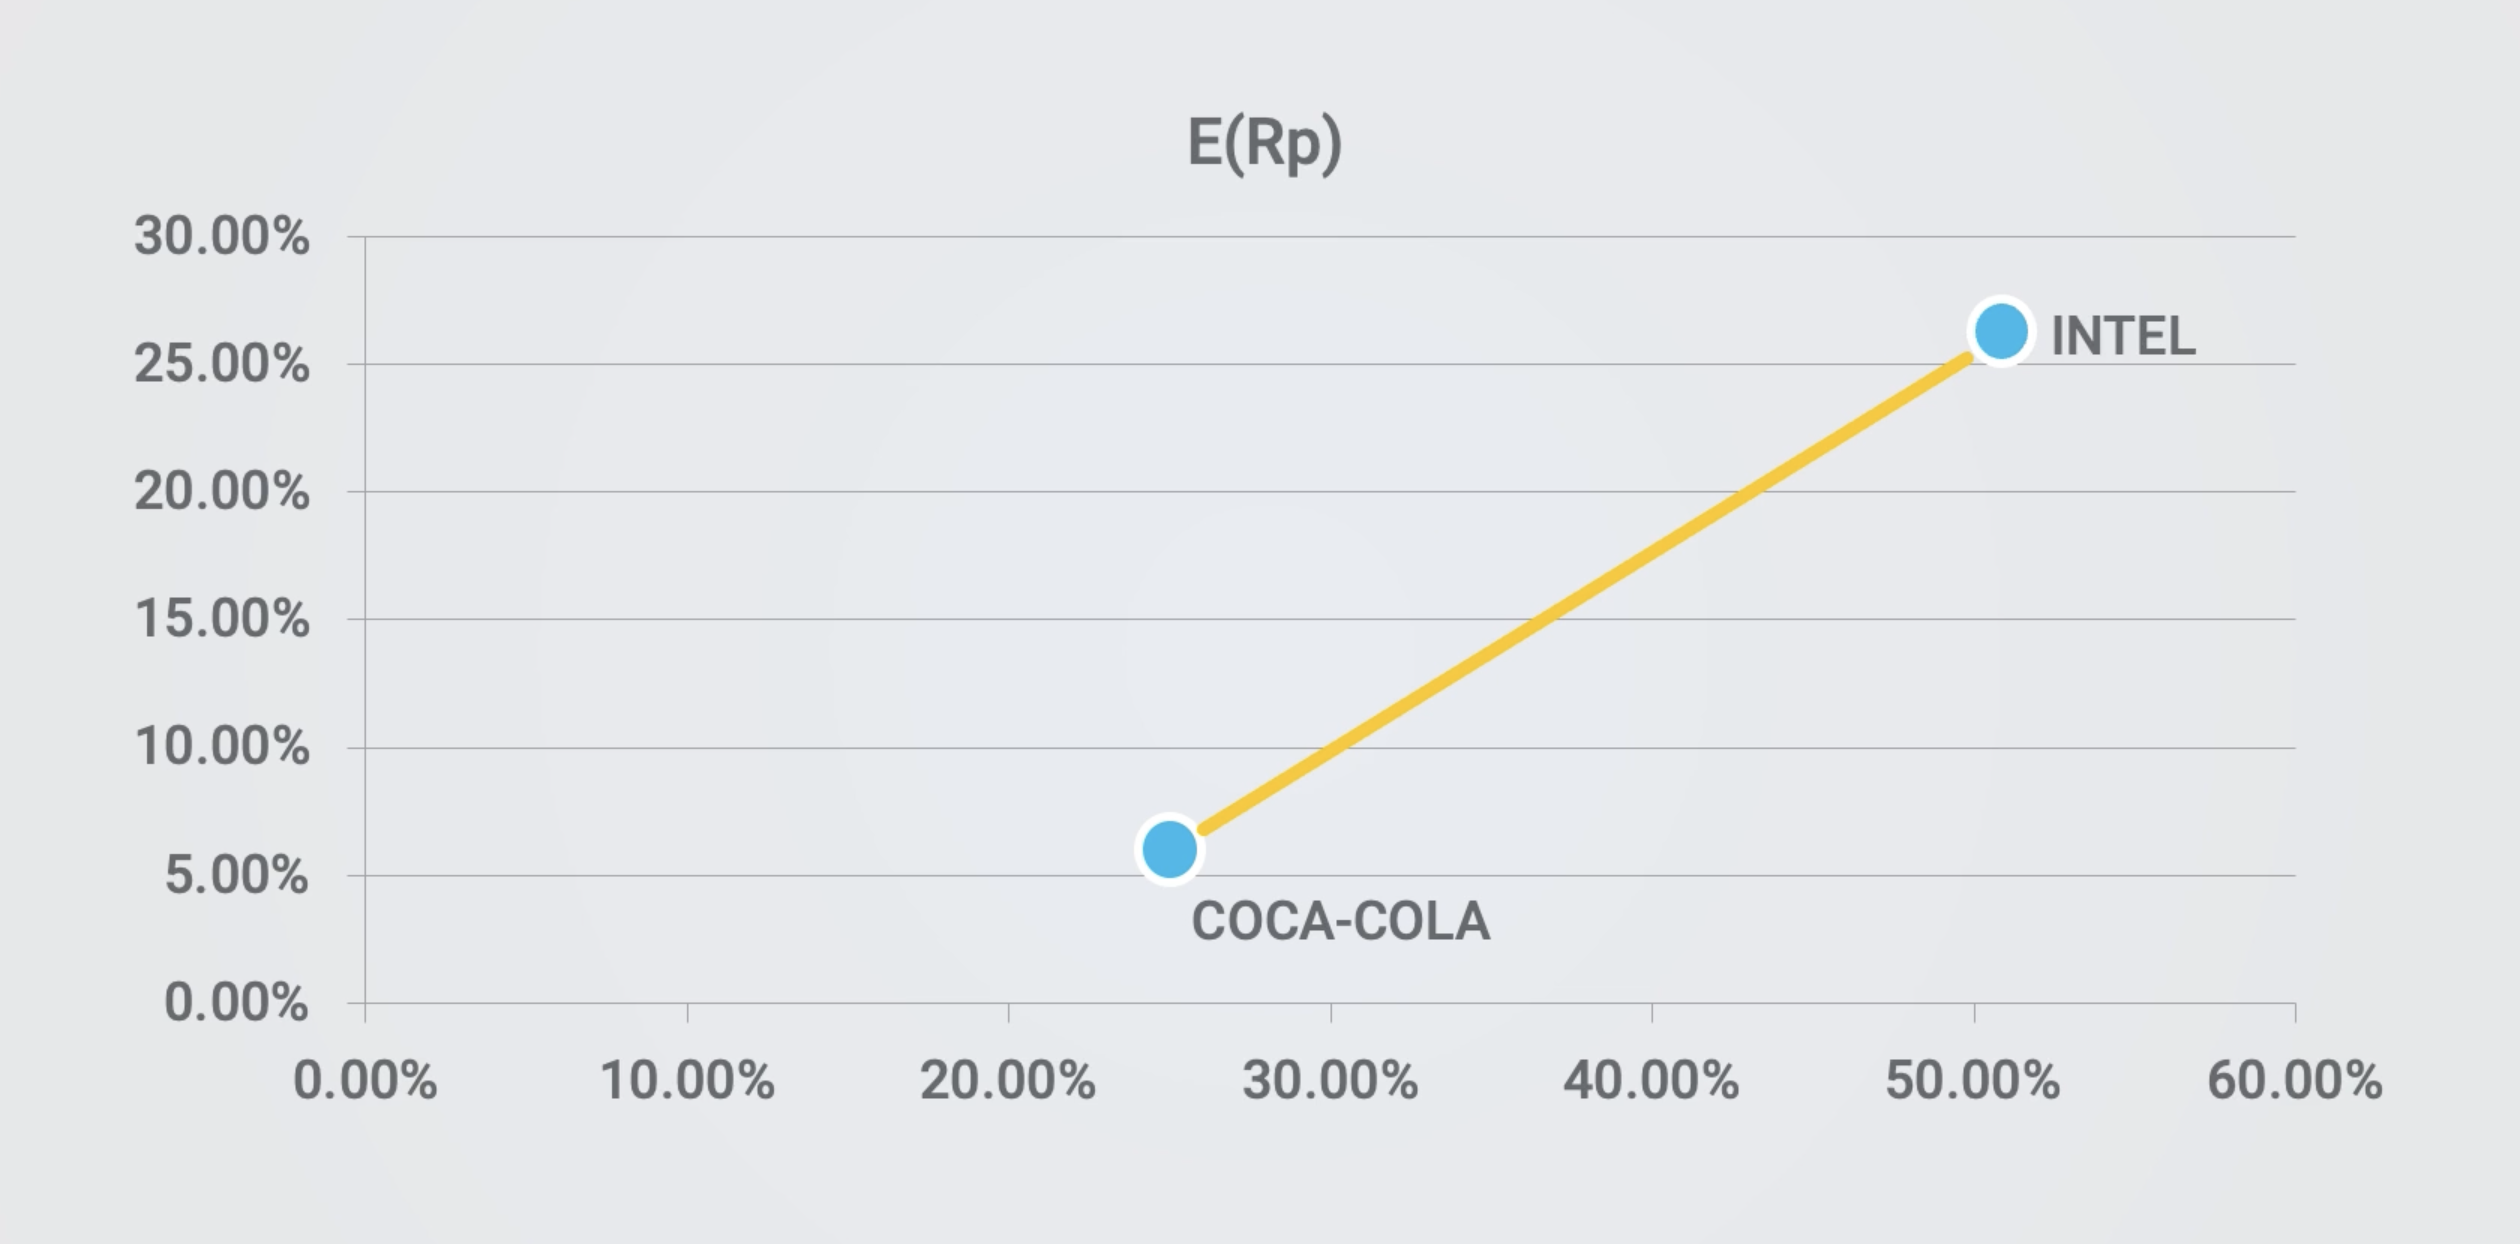
\includegraphics[width=0.8\textwidth]{img/6.2.2.png}
    \caption{Efficient Frontier if Intel and Coca-Cola have a correlation of 1}
    \label{fig:efficient_frontier_2}    
\end{figure}

If Intel and Coca-Cola have a correlation of 1, the efficient frontier will be a straight line, as the two assets move in the same direction. This means that there is no diversification benefit from holding both assets.\\

\begin{figure}[H]
    \centering
    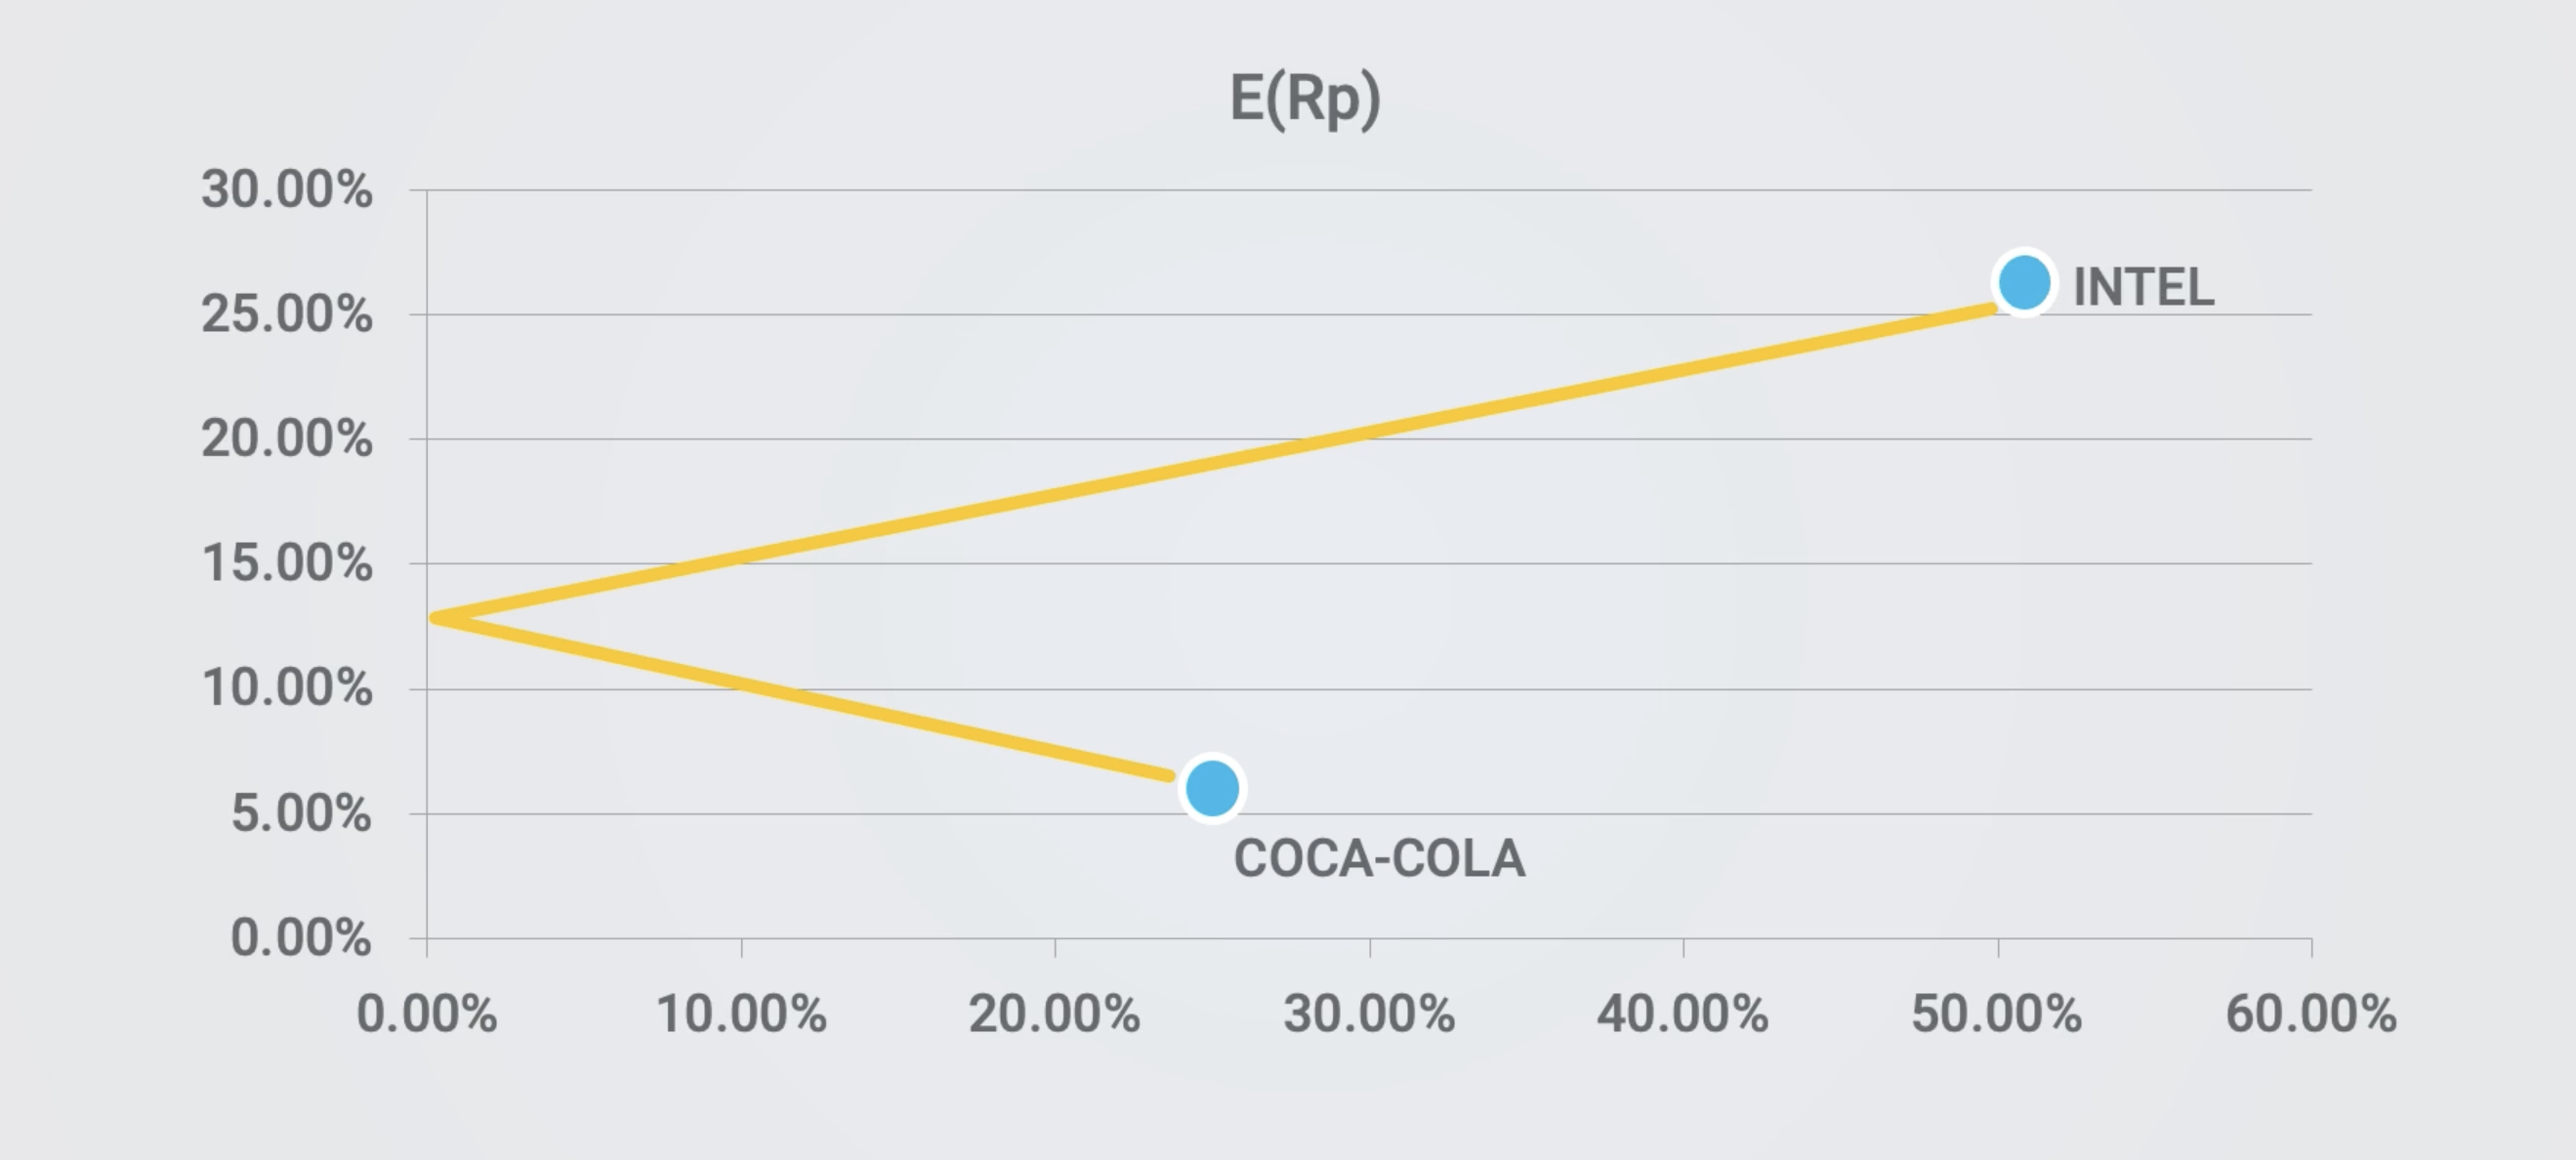
\includegraphics[width=0.8\textwidth]{img/6.2.3.png}
    \caption{Efficient Frontier if Intel and Coca-Cola have a correlation of -1}
    \label{fig:efficient_frontier_3}    
\end{figure}

If Intel and Coca-Cola have a correlation of -1, the efficient frontier will be a two-piece straight line, as the two assets move in opposite directions, so we can achieve a much lower risk for a given level of return.\\





\section{Principle of Diversification}

There are two components of total risk that investors face when investing:

\begin{enumerate}
    \item \textbf{Systematic Risk:} This is the risk that is inherent in the market that affects all companies, and cannot be diversified away. It is also known as market risk or non-diversifiable risk. Examples include interest rate risk, inflation risk, and political risk.
    
    \item \textbf{Idiosyncratic Risk:} This is the risk that is specific to a particular company or industry and can be diversified away. It is also known as idiosyncratic risk or diversifiable risk. It arises from factors that are specific to an individual asset or company, such as management decisions, competitive dynamics, operational issues, regulatory changes or even random events.  Examples include business risk, financial risk, and liquidity risk.
\end{enumerate}

In some asset pricing models like the CAPM, investors are compensated for taking on systematic risk, but not for idiosyncratic risk. This is because idiosyncratic risk can be diversified away by holding a diversified portfolio of assets.\\

\begin{figure}[H]
    \centering
    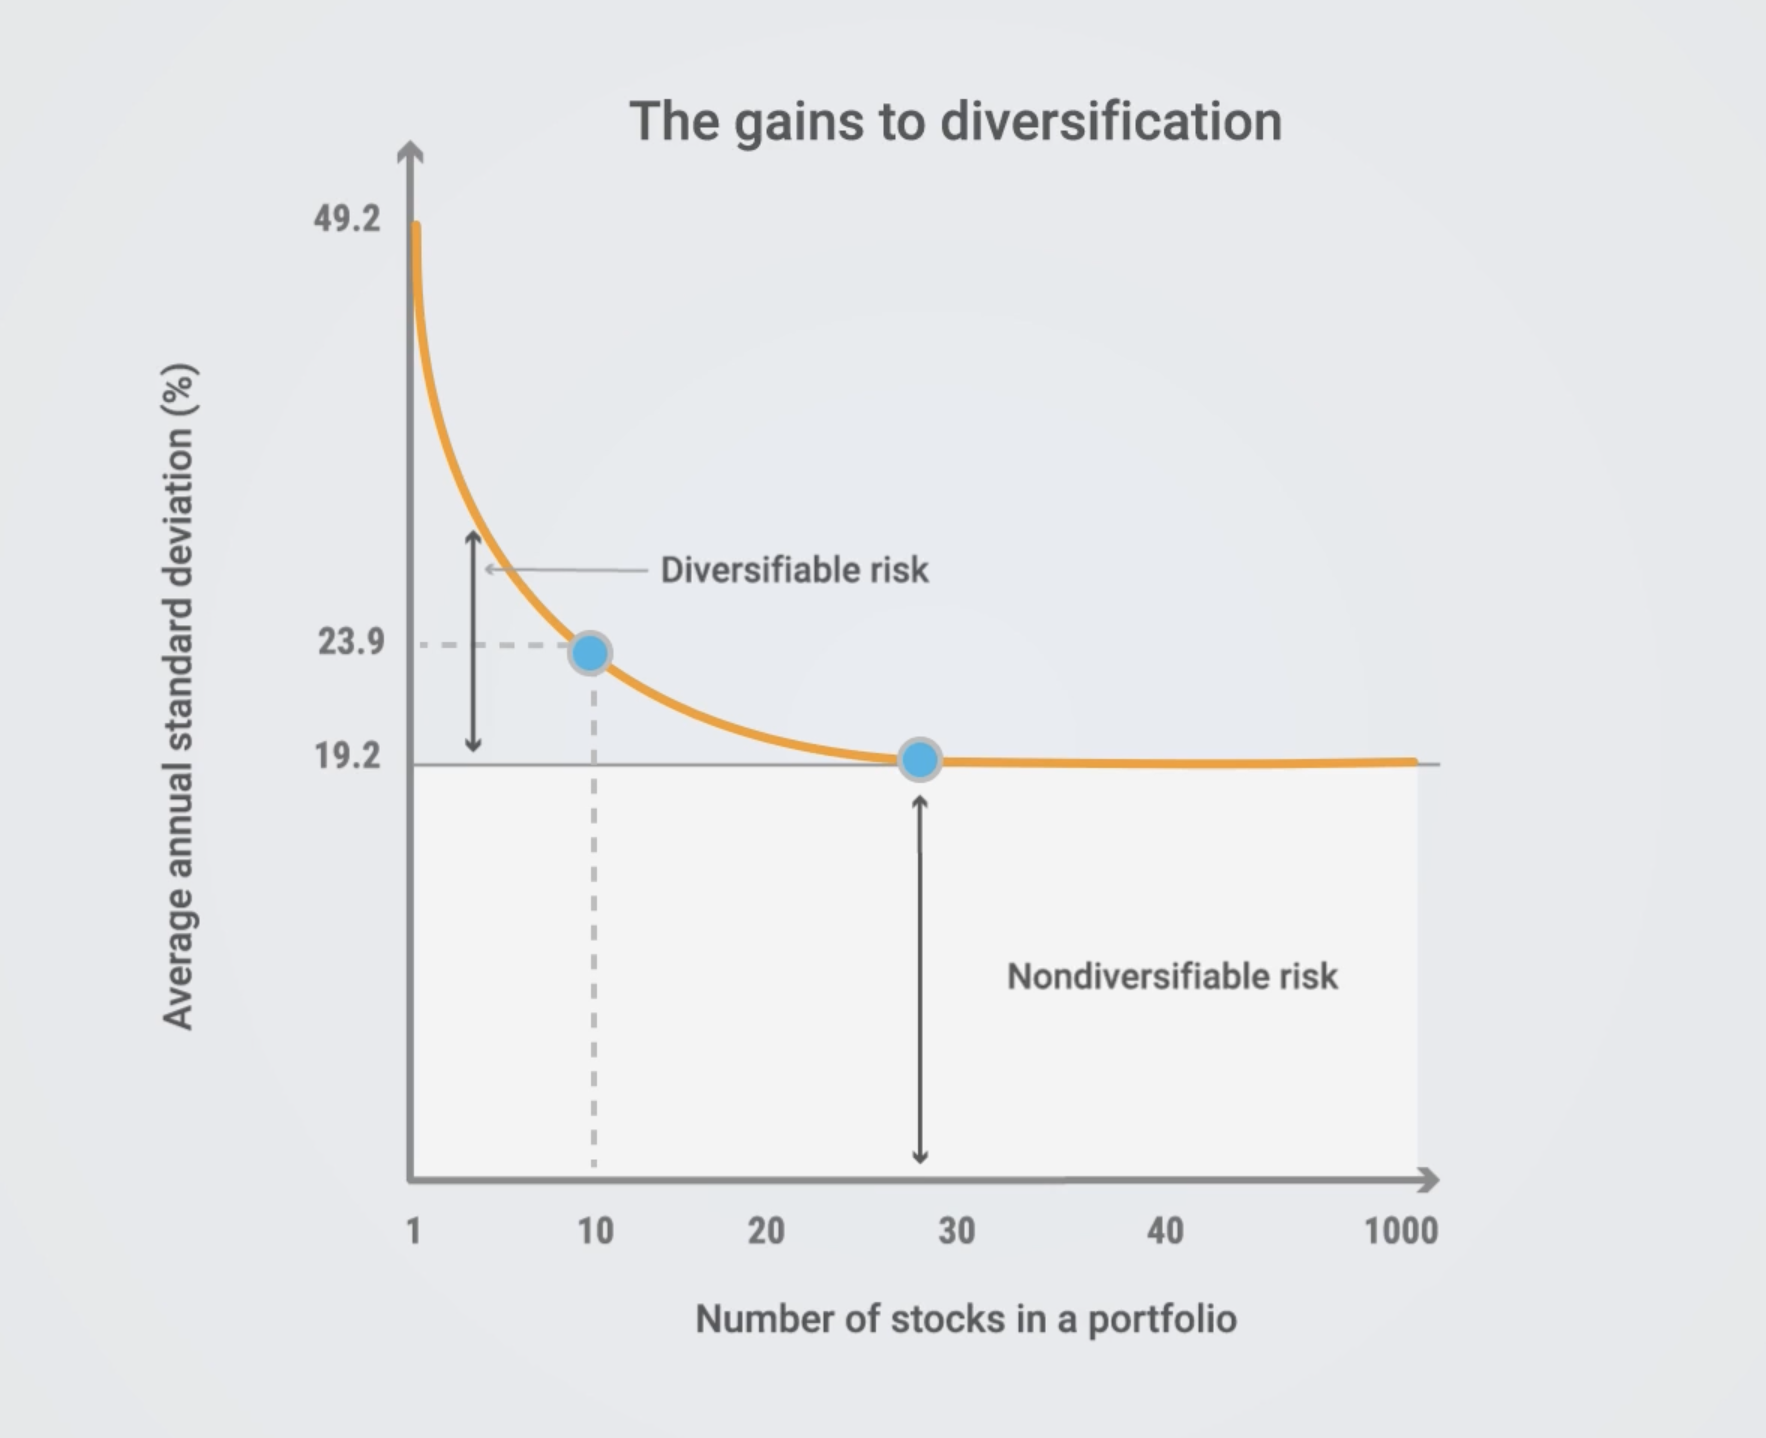
\includegraphics[width=0.5\textwidth]{img/6.2.4.png}
    \caption{Graph showing the diversifiable risk as the number of assets in a portfolio increases}
    \label{fig:diversified_risk}    
\end{figure}

\section{Measuring $\beta$}
\begin{itemize}
    \item A stock's beta, or $\beta$ is a measure of its sensitivity to market movements. 
    \item It is a measure of the stock's systematic risk, or the risk that cannot be diversified away. 
    \item A stock with beta $\beta=1$ in line with the market (identical changes in percentage).
    \item A stock with beta $\beta>1$ moves more than the market. (If the market goes up by 1\%, the stock goes up by more than 1\%)
    \item A stock with beta $0<\beta<1$ moves less than the market. (If the market goes up by 1\%, the stock goes up by less than 1\%)
    \item A stock with beta $\beta=0$ is uncorrelated with the market.
    \item A stock with beta $-1<\beta<0$ moves less than the market, but in the opposite direction. (If the market goes up by 1\%, the stock goes down by less than 1\%)
    \item A stock with beta $\beta=-1$ moves in the opposite direction of the market. (If the market goes up by 1\%, the stock goes down by 1\%)
    \item A stock with beta $\beta<-1$ moves more than the market, but in the opposite direction. (If the market goes up by 1\%, the stock goes down by more than 1\%)

\end{itemize}

\subsection*{The CAPM model}
The Capital Asset Pricing Model (CAPM) states that the expected return of a security is proportionate to its beta multiplied by the market risk premium. Beta is a measure of the security's systematic risk, and the market risk premium is the expected return of the market minus the risk-free rate. This is represented by the formula:

\begin{equation}
    E(R_i) = r_f + \beta_i(E(R_m) - r_f)
\end{equation}

Where:
\begin{itemize}
    \item $E(R_i)$ is the expected return of the security
    \item $r_f$ is the risk-free rate
    \item $\beta_i$ is the beta of the security
    \item $E(R_m)$ is the expected return of the market
    \item $E(R_m) - r_f$ is the market risk premium
\end{itemize}

It can be rewritten as:

\begin{equation}
    \frac{E(R_i) - r_f}{\beta_i} = \frac{E(R_m) - r_f}{\beta_m}
\end{equation}

This is the excess return of any security divided by its beta is consistent among all securities, where $\beta_m$ is the beta of the market which is equal to 1. So the reward for taking on risk is the same for all securities.\\

This forms the basis of an efficient market, where all securities are priced correctly according to their risk. If a security is priced too high or too low, investors will buy or sell the security until the price is correct.\\

\section{CAPM Graphically}
\begin{figure}[H]
    \centering
    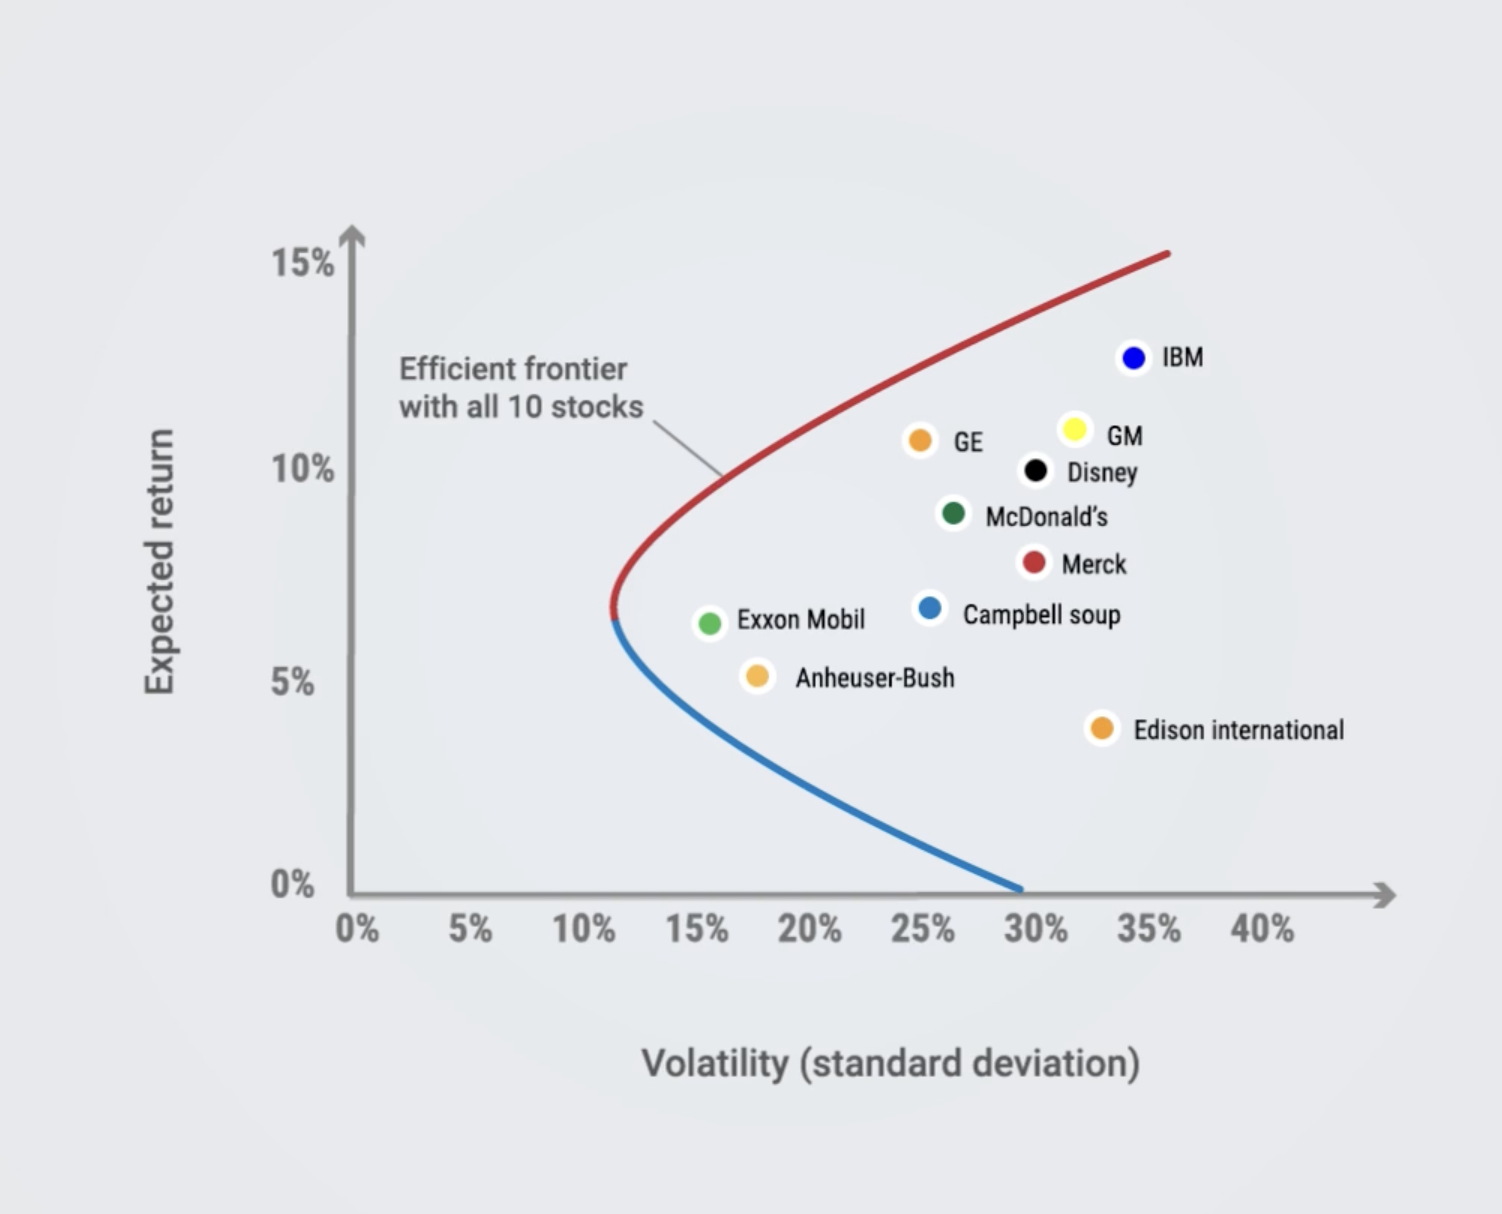
\includegraphics[width=0.6\textwidth]{img/6.5.png}
    \caption{Expected return over volatility, the efficient frontier.}
    \label{fig:capm_graph}
\end{figure}

Investors would only choose portfolios along the efficient frontier, as they offer the highest return for a given level of risk. 

We have a lot more combinations to create portfolios on light blue line, but not all are efficient. The CML is the most efficient portfolio of risky assets that an investor can hold, as it offers the highest return for a given level of risk.\\

\begin{itemize}
    \item Then this introduces the (new) efficient frontier coloured in green, the Capital Market Line (CML), containing the risk-free investment + other risky assets, separate from the efficient frontier that consists of only risky assets, coloured in red.
    \item There is also the market portfolio, that is tangential to combinations of risky assets and the risk-free asset. This market portfolio is the most efficient portfolio that contains only risk assets and no risk-free assets.
    \item The CML represents portfolios as a combination of the market portfolio (investment in risky assets only) and the risk-free asset.
    \item The expected return of a portfolio on the CML is given by the risk-free rate plus a risk premium proportional to the weight in the market portfolio. The volatility of these portfolios are proportional to the weight in the market portfolio (since the risk-free asset has no volatility).
\end{itemize}

\begin{figure}[H]
    \centering
    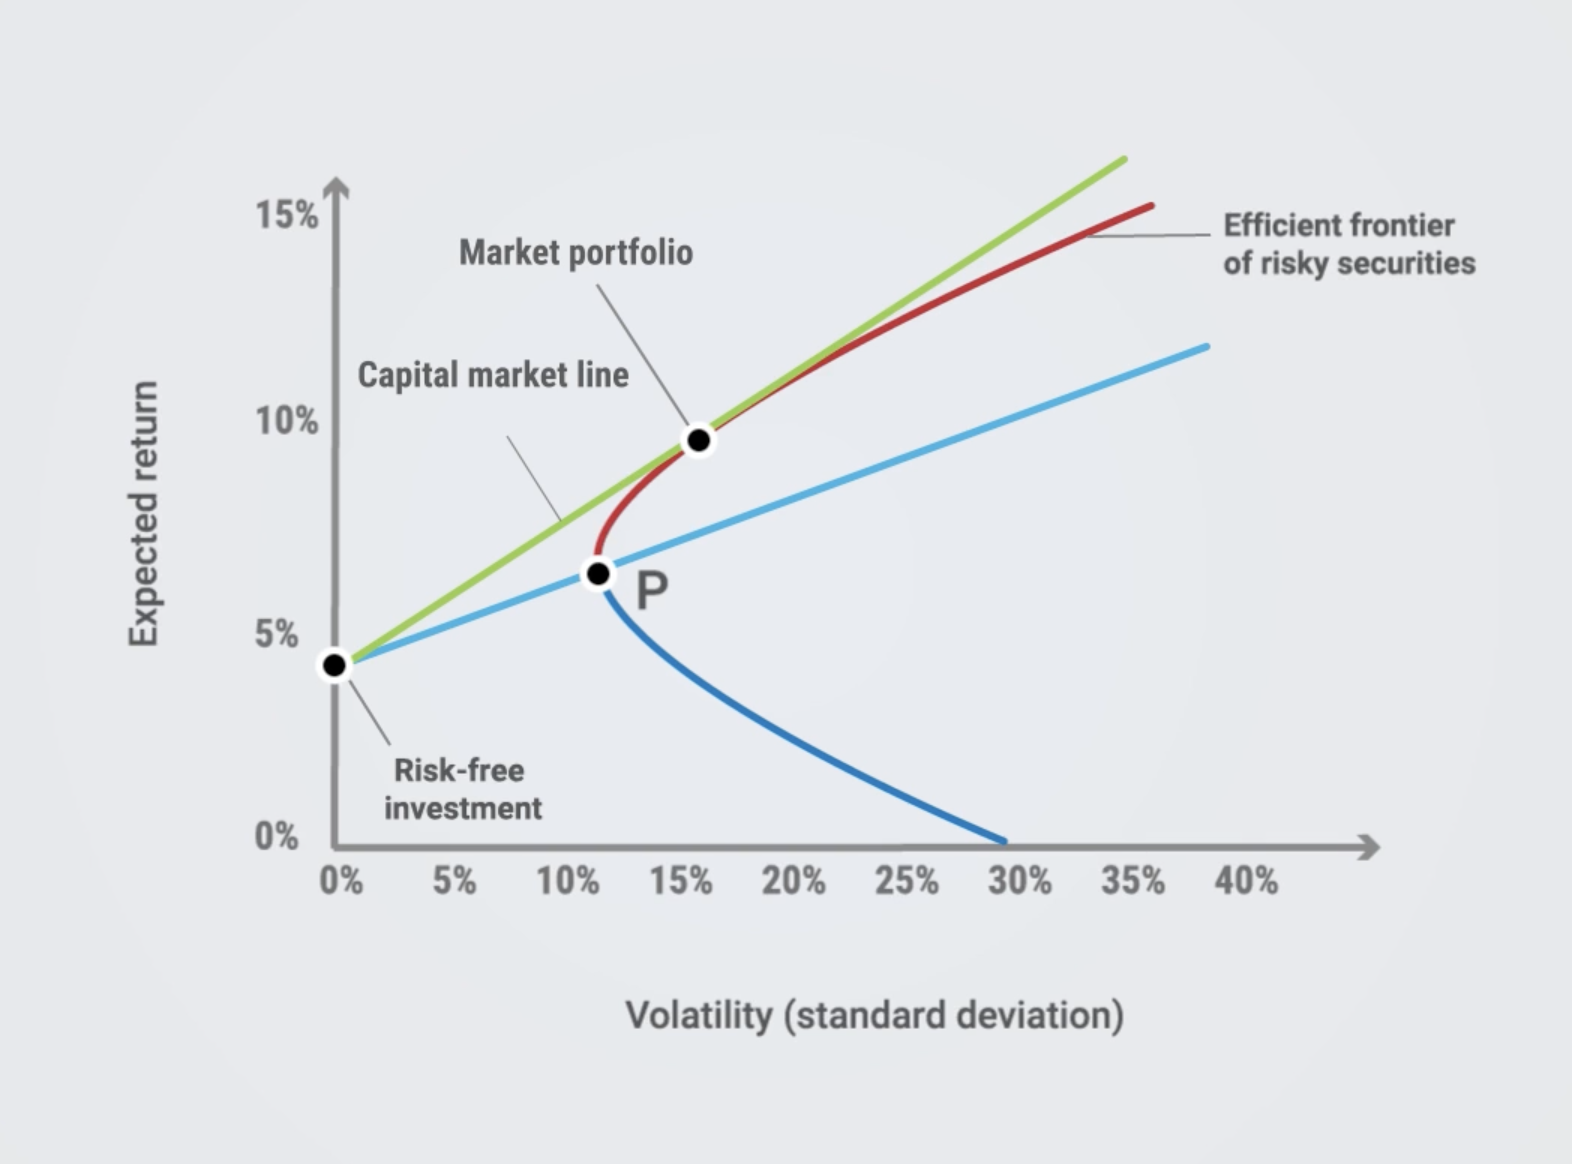
\includegraphics[width=0.6\textwidth]{img/6.6.png}
    \caption{Efficient Frontier and Capital Market Line}
    \label{fig:capm_graph_2}
\end{figure}

As for each individual stock, its level of expected return depends on its level of systematic risk as measured by beta. This relation is expressed graphically by the security market line, or SML.

\begin{figure}[H]
    \centering
    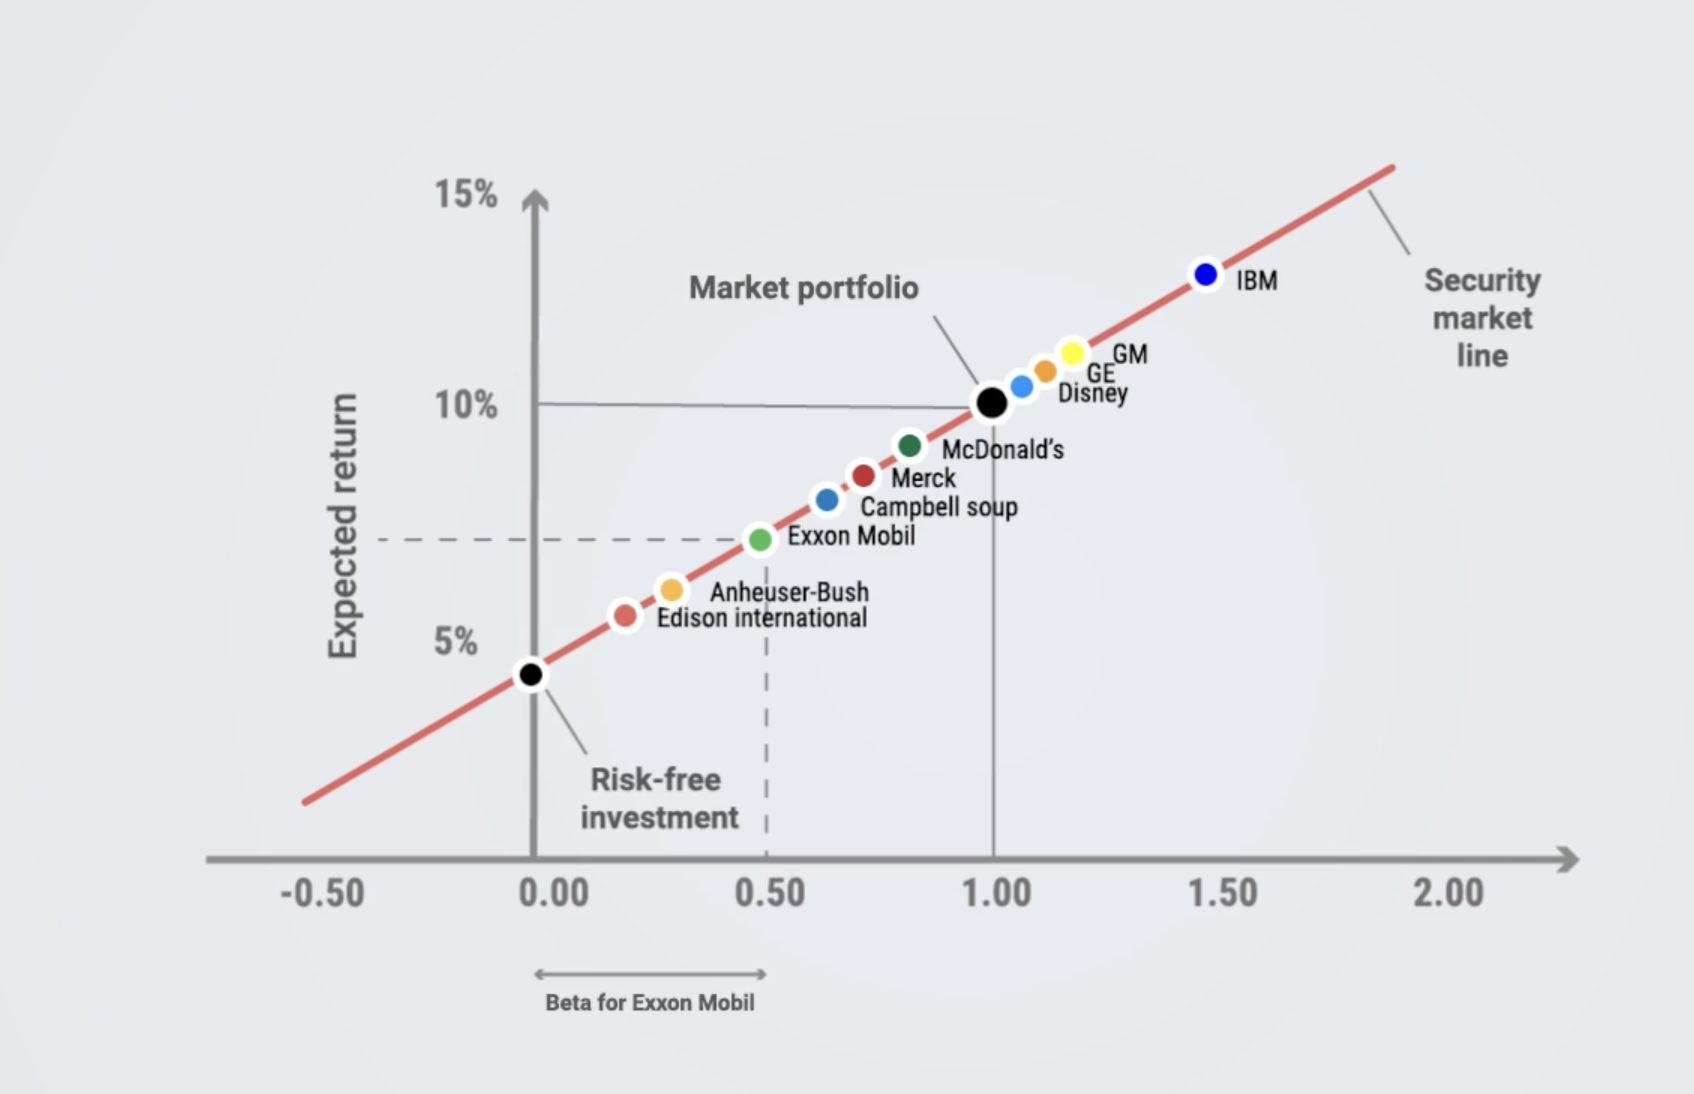
\includegraphics[width=0.6\textwidth]{img/6.7.png}
    \caption{Security Market Line}
    \label{fig:security_market_line}
\end{figure}


\section{Guest Speaker: Mike Kollo Interview}
In this video, Professor James Sefton interviews guest speaker Mike Kollo, who worked at AXA-Rosenberg at the time. They discuss Mike's work as an active portfolio manager.

\noindent \textbf{Key Points Discussed by Mike Kollo:}

\begin{itemize}
    \item \textbf{Market Efficiency and Crisis Impact:} Mike Kollo distinguishes between everyday market scenarios and crisis scenarios, like the 2008 financial crash. In normal conditions, markets integrate information such as earnings reports into prices with relative efficiency, particularly in well-covered, large markets. However, during crises, market dynamics change drastically, leading to rapid price changes and inefficiencies as traditional risk management approaches fail.
    
    \item \textbf{Active Management and Information Flow:} As an active portfolio manager at a quantitative asset management firm, Kollo emphasizes the importance of how information is integrated into market prices. His approach involves systematic analysis to incorporate new data into valuation models, helping predict market movements and enhance investment strategies.
    
    \item \textbf{Technological Advances and Data Integration:} The conversation also touched on the increasing role of technology in asset management. Kollo notes the challenge of filtering and using vast amounts of data effectively, including real-time data from unconventional sources like social media, to inform investment decisions.
    
    \item \textbf{Post-Crisis Industry Changes:} The financial crisis led to a shift in client expectations and industry practices. Investors are increasingly seeking low-volatility investments and outcome-based products. Asset management is moving towards more responsible and client-focused strategies, rather than purely profit-driven approaches.
    
    \item \textbf{Ethical and Educational Role of Asset Management:} Kollo suggests that the future of asset management could involve educating clients about risk and helping them understand the implications of their investments, thus shaping a more ethical and client-oriented industry.
\end{itemize}

\begin{commentbox}{Poll: Would you pay extra for an active portfolio manager?}
32\% answered No, 68\% answered Yes.\\

It is possible to construct a strategy that will outperform the market. For example, according to research mentioned in John H. Cochrane's New Facts in Finance, investing in smaller businesses has been shown to perform slightly better than the market. However, the market efficiency model explains 90-95\% of what is going on; hence, it is popular as a framework for understanding how markets function.\\

In efficient markets, all portfolios (when adjusted for risk) deliver the same return. But how can you adjust for risk? You need a model for this! And only then can you test it for market efficiency. At this point, though, if you do outperform the market, you cannot know for sure if it is because the market is inefficient, or whether your model is wrong. This is difficult to establish and this challenge has been prevalent for a long time!
\end{commentbox}